\documentclass{beamer}

\usepackage{default}
\usepackage[portuguese]{babel}
\usepackage[utf8]{inputenc}
\usepackage{graphicx}
\usepackage{hyperref}
\usepackage{mdwlist}
\usepackage{textcomp}
\usepackage{graphicx}
\usetheme{Antibes}


\title{Introdução à simulação de circuitos com o \textit{LTspice IV}}
\author{Renan Birck Pinheiro}
\institute{Universidade Federal de Santa Maria}

\begin{document}

\begin{frame}
\titlepage
\end{frame}

\begin{frame} % slide introdução
\frametitle{Introdução}
\begin{itemize}
\item{Por que simular circuitos?}
\begin{itemize}
\pause
\item{Complexidade do projeto de novos circuitos}
\pause
\item{Reduzir custos de prototipagem}
\pause
\item{Simplificar o processo de projeto}
\end{itemize}
\end{itemize}
\end{frame} % slide introdução

\begin{frame} % slide SPICE
\frametitle{SPICE}
\begin{itemize}
\item{\textbf{S}imulation \textbf{P}rogram \textbf{W}ith \textbf{I}ntegrated \textbf{C}ircuit \textbf{E}mphasis}
\item{\textbf{Primeiras versões}: anos 70, grandes computadores, modo texto}
\item{\textbf{SPICE 2}: anos 80/90, computadores de médio porte, interface gráfica}
\item{\textbf{Versões atuais}: computadores pessoais}
\pause
\item{\textbf{Vários fabricantes} pegaram o código e fizeram suas próprias versões adicionando recursos}
\begin{itemize}
\item{\textbf{Motivação}: atender interesses específicos de indústrias: microeletrônica, RF etc...}
\item{Assim, temos hoje diversos simuladores: PSpice, HSpice, LTspice, Proteus entre outros}

\end{itemize}
\end{itemize}
\end{frame} % slide SPICE

\begin{frame}
Vantagens:
\begin{itemize}
\item{Projeto} mais rápido, podem-se testar diversos componentes antes da compra.
\item{Medidas} que muitas vezes são difíceis de fazer na bancada.
\end{itemize}

\end{frame}

\begin{frame}
Desvantagens:
\begin{itemize}
\item{\textbf{Não substitui prototipagem:} os modelos dos componentes são idealizados, não levam efeitos térmicos ou as componentes parasitas da placa}
\item{\textbf{Necessidade} de modelos para os componentes}

\item{Em geral: \textbf{lixo entra, lixo sai}. Os resultados das simulações são tão bons quanto os modelos e o projeto do circuito forem.}
\end{itemize}
\end{frame}

\begin{frame}

\begin{figure}[htb]
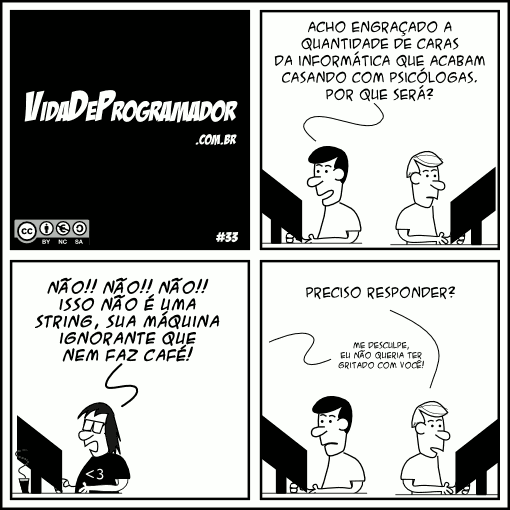
\includegraphics[width=200px]{images/tirinha33}
\caption{Lixo entra, lixo sai!}
\label{fig:lixoentrasai}
\end{figure}

\end{frame}

\begin{frame}
\frametitle{Desenhando um circuito}
\end{frame}

\begin{frame}
\frametitle{Componentes}
\end{frame}

\begin{frame}
\frametitle{Parâmetros: fontes de tensão}
\end{frame}

\begin{frame}
\frametitle{Análise transiente}
\begin{itemize}
\item{Análise no domínio do tempo, para circuitos lineares ou não}
\end{itemize}
\end{frame}

\begin{frame}
\frametitle{Exemplo 1: Circuitos RC e RLC}
\end{frame}

\begin{frame}
\frametitle{Análise AC}
\begin{itemize}
\item{Análise de pequenos sinais, no domínio da frequência}
\item{Circuitos não-lineares são \textbf{linearizados} ao redor do ponto de operação}

\item{As fontes são definidas como fasores com módulo e fase}
\item{Por exemplo: Fonte definida como \texttt{AC 1 0} = $1\measuredangle 0$} 
\end{itemize}
\end{frame}

\begin{frame}
\frametitle{Exemplo 2: Circuito com amplificador operacional}
\end{frame}

\begin{frame}
\frametitle{Análise de varredura DC}
\end{frame}

\begin{frame}
\frametitle{Exemplo 3: Amplificador \textit{common source}}
\end{frame}

\begin{frame}
\frametitle{Análise de Fourier}
\begin{itemize}
\item Permite visualizar o conteúdo harmônico de um sinal, isto é, as frequências que formam esse sinal.
\item \textbf{Sempre} especificar o parâmetro \textit{plotwinsize=0}, para desativar a compactação (que pode resultar na perda de componentes do sinal).
\end{itemize}
\end{frame}

\begin{frame}
\frametitle{Exemplo 4: Modulador AM a transistor}
\end{frame}

\begin{frame}
\frametitle{Resultados}
Da teoria de Fourier, que ao multiplicarmos um sinal de frequência $F_s$ por uma portadora de frequência $F_c$, obtemos as harmônicas $F_s + F_c$ e $F_s - F_c$. E isso fica visível no gráfico!
\end{frame}


\begin{frame}
\frametitle{Medição de THD com Fourier}
\end{frame}

\begin{frame}
\frametitle{Exemplo 5: Amplificador \textit{push-pull}}
\end{frame}

\begin{frame}
\frametitle{Links de interesse}
\begin{itemize}
\item \url{http://tech.groups.yahoo.com/group/LTspice/} - grupo de usuários do LTspice
\end{itemize}
\end{frame}


\begin{frame}
{\LARGE OBRIGADO!}
\end{frame}

\begin{frame}
Contatos: \url{renan.ee.ufsm@gmail.com} \url{http://facebook.com/renanbirck} \url{http://twitter.com/renan2112}\newline
O código-fonte desses slides e os circuitos empregados estão disponíveis em \url{https://github.com/renanbirck/minicurso-2012} ou com o autor.

\end{frame}
\end{document}
